\documentclass[a4paper,12pt]{article}
\usepackage[utf8]{inputenc}
\usepackage[english]{babel}
\usepackage{graphicx}
\usepackage{amsmath}
\usepackage{amssymb}
\usepackage{hyperref}
\usepackage{geometry}
\geometry{a4paper, left=25mm, right=25mm, top=25mm, bottom=25mm}

\title{Project 1: Supervised Learning - Classification}
\author{To be filled in}
\date{\today}

\begin{document}

\maketitle

\begin{abstract}
Placeholder
\end{abstract}

\section{Introduction}
Placeholder

\begin{figure}[h]
    \centering
    % Platzhalter für die Abbildung
    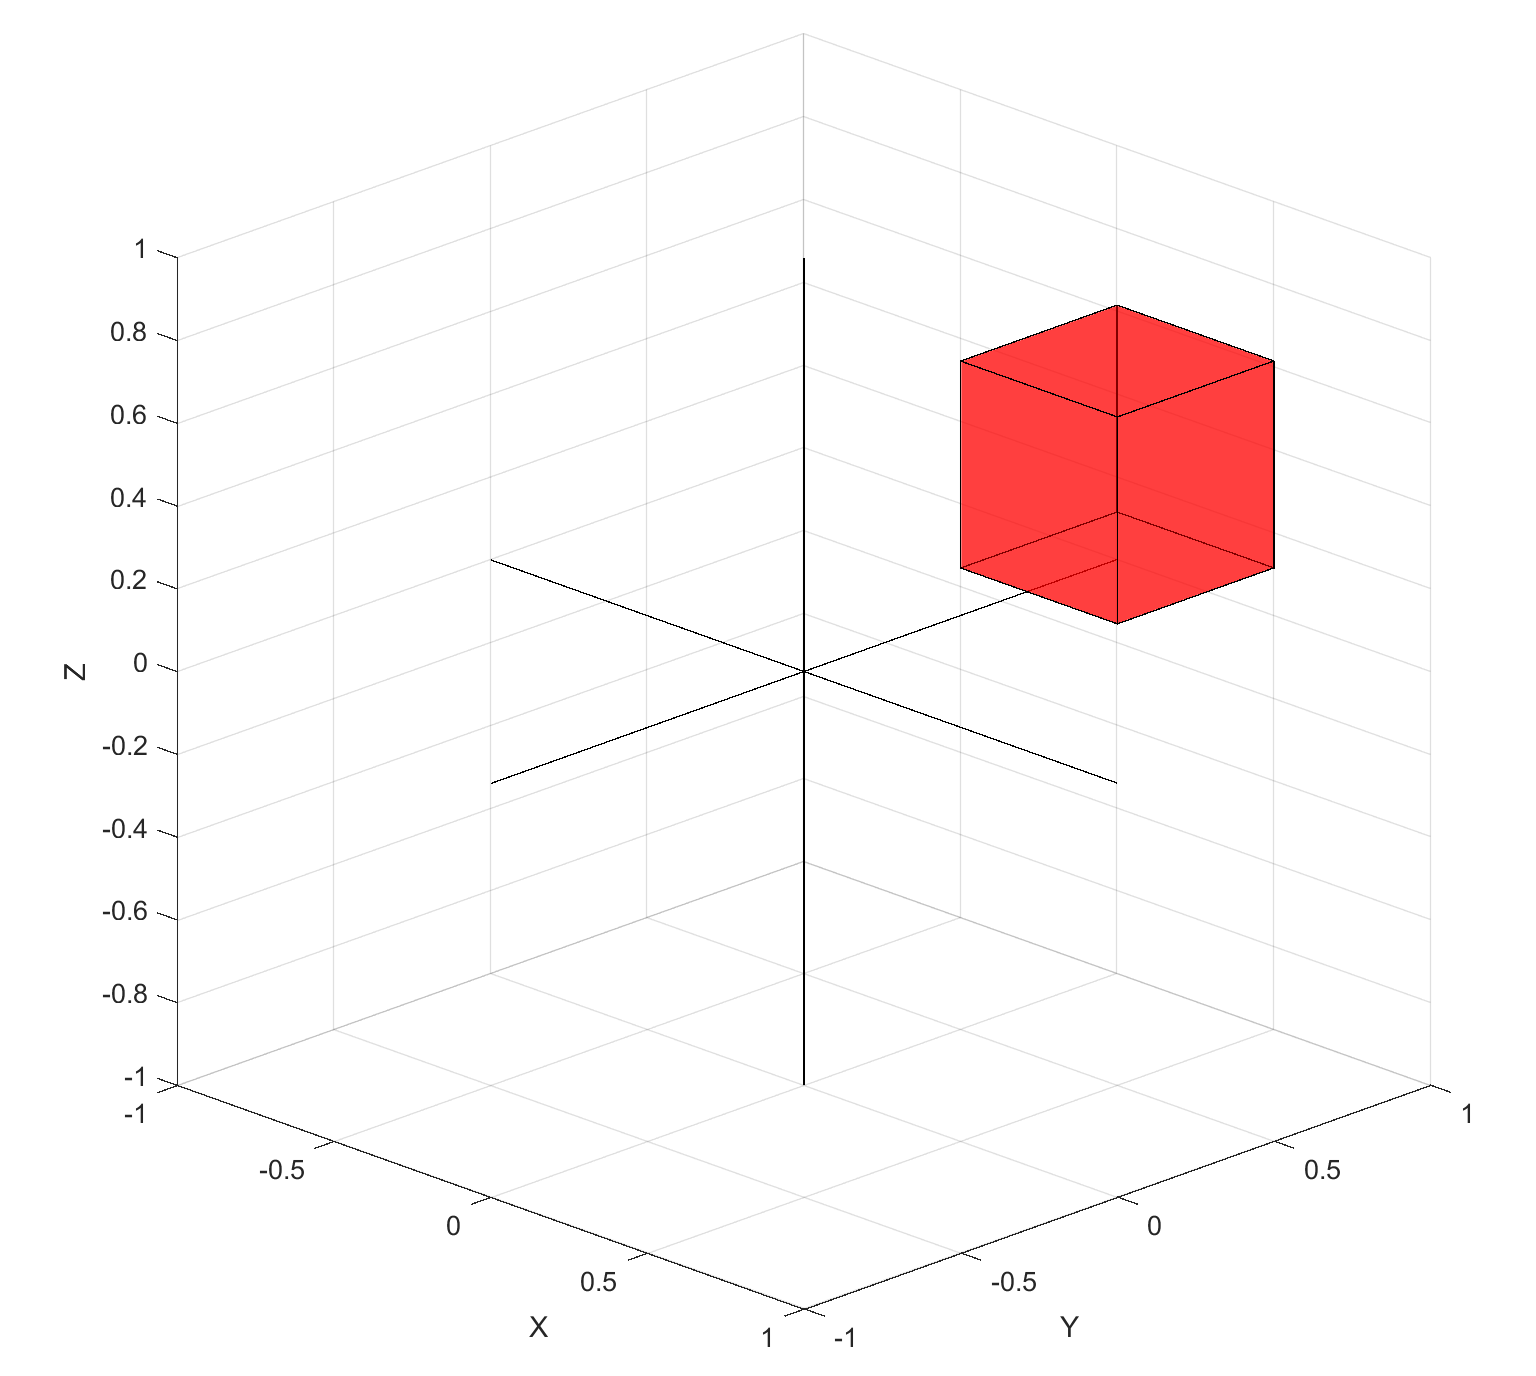
\includegraphics[width=0.5\textwidth]{cube.png}
    \caption{Cube \( W = \{\mathbf{v}: v_x, v_y, v_z
\in [0.25, 0.75] \} \) with center \( (0.5, 0.5, 0.5)^T\)}
    \label{fig:Introduction}
\end{figure}

Some formula:
\[ \mathbf{-t} + (\mathbf{R_z} \cdot (\mathbf{t} + \mathbf{v} )) = 
    (\mathbf{R_z}\mathbf{t} - \mathbf{t}) + (\mathbf{R_z}\mathbf{v})\]


\section{Process}
Placeholder

\subsection{Subparagraph}
Placeholder

\section{Results}
Placeholder

\section{Conclusions}
Placeholder

\section{Future Work}
Placeholder


\clearpage

\section{Sources}

\begin{itemize}
    \item some source
\end{itemize}

\end{document}
